% Options for packages loaded elsewhere
\PassOptionsToPackage{unicode}{hyperref}
\PassOptionsToPackage{hyphens}{url}
%
\documentclass[
]{article}
\usepackage{lmodern}
\usepackage{amsmath}
\usepackage{ifxetex,ifluatex}
\ifnum 0\ifxetex 1\fi\ifluatex 1\fi=0 % if pdftex
  \usepackage[T1]{fontenc}
  \usepackage[utf8]{inputenc}
  \usepackage{textcomp} % provide euro and other symbols
  \usepackage{amssymb}
\else % if luatex or xetex
  \usepackage{unicode-math}
  \defaultfontfeatures{Scale=MatchLowercase}
  \defaultfontfeatures[\rmfamily]{Ligatures=TeX,Scale=1}
\fi
% Use upquote if available, for straight quotes in verbatim environments
\IfFileExists{upquote.sty}{\usepackage{upquote}}{}
\IfFileExists{microtype.sty}{% use microtype if available
  \usepackage[]{microtype}
  \UseMicrotypeSet[protrusion]{basicmath} % disable protrusion for tt fonts
}{}
\makeatletter
\@ifundefined{KOMAClassName}{% if non-KOMA class
  \IfFileExists{parskip.sty}{%
    \usepackage{parskip}
  }{% else
    \setlength{\parindent}{0pt}
    \setlength{\parskip}{6pt plus 2pt minus 1pt}}
}{% if KOMA class
  \KOMAoptions{parskip=half}}
\makeatother
\usepackage{xcolor}
\IfFileExists{xurl.sty}{\usepackage{xurl}}{} % add URL line breaks if available
\IfFileExists{bookmark.sty}{\usepackage{bookmark}}{\usepackage{hyperref}}
\hypersetup{
  pdftitle={Examining the Impact of Covid-Shutdown on Toronto Restaurants Paper},
  pdfauthor={Youjing Li, Ken Lee, Renjing Liu, Jialin Zhao},
  hidelinks,
  pdfcreator={LaTeX via pandoc}}
\urlstyle{same} % disable monospaced font for URLs
\usepackage[margin=1in]{geometry}
\usepackage{longtable,booktabs}
\usepackage{calc} % for calculating minipage widths
% Correct order of tables after \paragraph or \subparagraph
\usepackage{etoolbox}
\makeatletter
\patchcmd\longtable{\par}{\if@noskipsec\mbox{}\fi\par}{}{}
\makeatother
% Allow footnotes in longtable head/foot
\IfFileExists{footnotehyper.sty}{\usepackage{footnotehyper}}{\usepackage{footnote}}
\makesavenoteenv{longtable}
\usepackage{graphicx}
\makeatletter
\def\maxwidth{\ifdim\Gin@nat@width>\linewidth\linewidth\else\Gin@nat@width\fi}
\def\maxheight{\ifdim\Gin@nat@height>\textheight\textheight\else\Gin@nat@height\fi}
\makeatother
% Scale images if necessary, so that they will not overflow the page
% margins by default, and it is still possible to overwrite the defaults
% using explicit options in \includegraphics[width, height, ...]{}
\setkeys{Gin}{width=\maxwidth,height=\maxheight,keepaspectratio}
% Set default figure placement to htbp
\makeatletter
\def\fps@figure{htbp}
\makeatother
\setlength{\emergencystretch}{3em} % prevent overfull lines
\providecommand{\tightlist}{%
  \setlength{\itemsep}{0pt}\setlength{\parskip}{0pt}}
\setcounter{secnumdepth}{5}
\ifluatex
  \usepackage{selnolig}  % disable illegal ligatures
\fi
\newlength{\cslhangindent}
\setlength{\cslhangindent}{1.5em}
\newlength{\csllabelwidth}
\setlength{\csllabelwidth}{3em}
\newenvironment{CSLReferences}[2] % #1 hanging-ident, #2 entry spacing
 {% don't indent paragraphs
  \setlength{\parindent}{0pt}
  % turn on hanging indent if param 1 is 1
  \ifodd #1 \everypar{\setlength{\hangindent}{\cslhangindent}}\ignorespaces\fi
  % set entry spacing
  \ifnum #2 > 0
  \setlength{\parskip}{#2\baselineskip}
  \fi
 }%
 {}
\usepackage{calc}
\newcommand{\CSLBlock}[1]{#1\hfill\break}
\newcommand{\CSLLeftMargin}[1]{\parbox[t]{\csllabelwidth}{#1}}
\newcommand{\CSLRightInline}[1]{\parbox[t]{\linewidth - \csllabelwidth}{#1}\break}
\newcommand{\CSLIndent}[1]{\hspace{\cslhangindent}#1}

\title{Examining the Impact of Covid-Shutdown on Toronto Restaurants Paper}
\author{Youjing Li, Ken Lee, Renjing Liu, Jialin Zhao}
\date{19 二月 2021}

\begin{document}
\maketitle

\newpage

\hypertarget{introduction}{%
\section{Introduction}\label{introduction}}

Local businesses, especially restaurants, are the soul of many cities, providing not just a source of food, but also culinary diversity, culture, and employment for the population. In fact, these restaurants are vital contributors to the local community, donating to food banks, hosting fundraisers, and much more. Hence, with the presence of COVID-19, it is clear why the Ontario government would want to understand more about the potential effects a shutdown could have on the restaurants. Nevertheless, limiting the spread of this virus should be a top priority, but shutting down restaurants could have an immense effect on the local community, and hence affect the livelihoods of many Ontario residents. After all, many other factors have already had an adverse impact on the restaurant industry. For instance, studies like the ``COVID-19 and restaurant demand: Early effects of the pandemic and stay-at-home orders'' (Yang Yang 2020) have shown that a 1\% increase in new COVID cases results in 0.0556\% of daily restaurant demand, while stay-at-home orders have been associated with a decrease of 3.30\% in restaurant demand.

Therefore, this paper will focus on examining the effects of COVID shutdowns on restaurants, taking into account factors such as the net profit/loss of the businesses, the permanent closure of the restaurant, number of employees, wages, and food price. After all, shutting down a restaurant does not just affect the restaurant owners, as people may lose their jobs, have their wage/salary decrease, and prices for food may increase to compensate for losses.

For this research, we will first describe the intervention of this experiment where randomized controlled trial testing will be conducted on a sample of the restaurant population in Ontario. The methodology involved will then be defined, illustrating how we will be observing the restaurants, what will be measured, the population and sample of the experiment, and the predicted cost of gathering the data. At last, upon denoting all the details of our experiment's intervention method and survey methodology, we will be exploring our findings of the effects of COVID shutdowns on restaurants in the discussion section. All in all, this study will highlight the potential losses in profits and employment caused by restaurant shutdowns, helping Ontario government officials make better-informed decisions regarding the COVID restrictions such as shutdowns.

\newpage

\hypertarget{experiment-design}{%
\section{Experiment Design}\label{experiment-design}}

\hypertarget{intervention}{%
\subsection{Intervention}\label{intervention}}

We are going to implement our intervention in Ontario. Based on (Paul J. Gertler 2016), we used before-and after comparisons method to compare the outcomes of the same group of restaurants before and after the intervention within a two-month period from April 2021 to May 2021 to help the client understand the impact of COVID shut-downs on restaurant businesses.

We first extract a list of 32499 restaurants operating in the Ontario area from Yelp API as the frame, and then apply the stratified sampling method to divide the restaurants into different subgroups(strata) based on common attributes: price, rating, location and the number of reviews into different subgroups and the collection of all strata could fully represent the population which in our case is the restaurant business in the Ontario area. Then we implement the simple random sampling strategy to select an equal number of sample restaurants from each of the subgroups. Based on (BYJU's 2021), we used the equation below to calculate the sample size.

\begin{equation}
n= \frac{\frac{Z^2 \bullet p(1-p)}{e^2}}{1+(\frac{Z^2\bullet p(1-p)}{e^2N})} \label{eq:sampleSize}
\end{equation}

Where \[Z\] is the z score;
\[e\] is the margin of error;
\[N\] is the population size;
\[p\] is the population proportion;
\[n\] is the sample size

To carry out this calculation, we set the margin of error, \[e\], the maximum distance desired for the sample estimated to deviate from the true value, to be 5\%. The confidence level, which is a measure of certainty regarding how accurately a sample reflects the population, is set to be 0.95. \[Z\] for a 95\% confidence level is 1.96. The population proportion, denoted by \[p\], is set to be 0.5, describing a percentage value associated with a population. Thus, the sample size is calculated as 380, which means 380 or more restaurants are needed to have a confidence level of 95\% that the real value is within \[\pm\]5\% of the surveyed value. These 380 restaurants will be the target of our intervention and survey.

The stratified sampling technique helps to generate a more equal representation of characteristics in the sample group since we classify their features before distributing them directly into control and intervention groups, and also to maintain a lower sampling error in estimation, as well as a lower standard deviation. Therefore, any variations of outcomes between the control and treatment groups could be considered by the intervention only.
The next step of this study is to find two months in the year where restaurants are historically proven to have similar performances and then separating the control group and the treatment in our intervention. This will allow us to measure their usual performance and avoid counterfeit counterfactual mistakes.

To do so, we found the monthly survey of food services and drinking places dataset contains aggregated data of monthly sales amount for restaurants in different geographies since 1998 (S. Canada 2020). We filtered the dataset to only the geography as Ontario, and limited the time period from 2016 to 2019. There were 47 observations in the dataset and 3 attributes: month, the year of that month and Total Sales. An additional attribute to reflect monthly sales change was created during analysis by subtracting the total sales of the current month from the total sales of the previous month, and divided by the latter. The observations were aggregated by different months, we then calculated the average sales change in each month. \ref{fig:fig20}) below compares the average percentage change (compared with the previous month) of Ontario's restaurant monthly sales across different months from 2016 to 2019. The result indicates restaurants in Ontario have the most similar business performances in April and May.

\begin{figure}
\centering
\includegraphics{Examining-the-Impact-of-Covid-Shutdown-on-Toronto-Restaurants-Paper_files/figure-latex/fig20-1.pdf}
\caption{\label{fig:fig20}Ontario's restaruants business performances}
\end{figure}

Based on that, April and May are finally given as our options. The selected group of restaurants in April will be our control group (Group A), which will not be shut-down. The treatment (Group B) will be the selected group of restaurants in May, which will be shut-down. According to (Paul J. Gertler 2016), we believe our treatment and comparison group are the same in at least 3 ways: 1. On average characteristics of treatment and comparison groups should be the same, as restaurants' performances in April and May are historically proven very similar, restaurants in Group A and Group B are completely same. 2. The treatment should not affect the comparison group either directly or indirectly, as the control group (Group A) occurs before the treatment (Group B). 3. The outcomes of units in the control group should change the same way as outcomes in the treatment group. As a result, the differences between the two groups can only be explained by the existence of shut-down intervention.

We develop three key metrics to measure the business performance of restaurants in each group, profit or loss can reflect the tendency of restaurant turnovers, business renewals can indicate whether the restaurants plan to continue their business or not, employment will reflect the basic situation of the restaurant labor force. At the end of each month, our survey will be used to collect all the information mentioned above.

\hypertarget{methodology}{%
\subsection{Methodology}\label{methodology}}

The survey is generated using Microsoft Forms and is set to only one response per user to avoid duplicate responses. In addition, the survey includes an explanation of the experiment, denoting how the experiment will be conducted and upcoming surveys that they would still need to fill out in the following two months. For instance, it would explain how they would be allowed to operate normally in the first month, but some may be randomly picked to be shut-down in the second month. Of course, it would also indicate the compensation that would be given to them for shutting down (while also specifying that the compensation would not form part of the restaurant's revenue as to not intervene with the experiment). Additionally, we will be assuring the participants that their data would ultimately be anonymous and stored safely for their privacy, ensuring there are no privacy concerns and increasing the response rate. After all, the research data we collect from responsive surveys will fall under the Municipal Freedom of Information and Protection of Privacy Act(Information and Ontario 2015). Personal information such as the respondent's location, or opinions will be encoded into different classifications to hide sensitive personal information, and also the survey will be conducted anonymously to ensure all information is handled in a de-identified manner. The information we collect, use and analyze will not disclose to any third-party and only for research-purpose which comply with privacy protection provisions of the Acts. At last, the survey explanation would also include the importance of this study as it could inform government plans regarding how restaurants' laws are imposed. This would encourage respondents to answer the surveys, reducing the non responses. Of course, we made sure to state that their responses would not directly affect, but just inform government decisions, as some respondents may want to answer dishonestly to affect potential governmental outcomes.

More specifically, since we obtain detailed information for these 380 selected sample restaurants, such as email and phone number through Yelp API, the survey will first be conducted through an email survey, where we attach and send the survey link to associated email contact manually and respondents would be given a chance to opt-out of the study, preventing further contact from us. Nevertheless, upon a non-response, a similar follow-up email survey will be sent to reduce non-responses. Again, this survey would give the respondent a second chance to opt-out of this study. At last, if the emails garner no responses, a final phone call survey would be implemented to further reduce non-responses. These email and phone surveys will help us obtain information about each restaurant in these two control and treatment groups after performing the stratified sampling technique for the target population. The survey methodology process would be repeated three times, before the first month to provide the purpose of the experiment and options to opt-out/opt-int, at the end of the first month to have an idea (benchmark) of their usual performance, and at the end of the final month to evaluate the performance of the restaurants after treating half of them with lockdowns. Additionally, respondents will also be informed in the first survey that they will be rewarded after completing all three surveys with an incentive(such as Amazon gift cards) in order to achieve a higher response rate (a track record of the responses would be used to make sure restaurants do not send in two surveys and receive more than one gift card). If any of the restaurants that participated in the first survey decide not to participate in the upcoming surveys, they will not be able to obtain a gift card, and their previous data points in the past survey would be omitted. In fact, since we could not guarantee each respondent will take the survey eventually, weight-class adjustments will be implemented by increasing the sampling weights of respondents to manage the variation caused by unit nonresponses, in order to help us deal with non-response bias which could affect the validity of the research analysis and lead to an underestimation or overestimation of the true outcome.

The construction of the survey itself will be free with the Microsoft Forms platform and we will conduct the survey through email and phone only in which there will be no cost for sending email survey but an extra expense of calling non-response participants is required. Since the survey will be implemented in April and May, a two-month prepaid phone plan from Koodo mobile which is 25 CAD(\$) per month with unlimited province-wide calling will be purchased. In addition, each respondent will be rewarded with a 10 \$ Amazon gift card after completing all three surveys and the selected sample group for the survey is around 380. The estimated cost of conducting the survey is about 3850 \$ for each city where 3800 \$ will be used for purchasing Amazon gift cards(10 \$ gift card for each respondent), and 50 \$ is the payment for a two-month prepaid phone plan(25 \$ per month). Applying a risk factor of 15\% and setting the number of sampled cities to 5, a total cost of \$22137 is estimated to provide flexibility in budgets and to accommodate cases where more respondents are sampled. Labour costs are factored out of the costs since Petit Poll is a non-profit organization.

\newpage

\hypertarget{survey-design}{%
\section{Survey Design}\label{survey-design}}

As discussed in Section 2 Experiment Design, in order to determine how restaurants are coping with COVID-19 in Ontario, a survey is required to collect data pertaining to restaurant operations, finances, and staffing. The short survey consists of 10 questions (see Appendix I) and targets the government's major concerns---revenue shifts, labour changes, and business survivals; these topline metrics are collected from individual restaurants along with differentiating business characteristics such as size of business, source of debt, current operation status, Yelp star rating, number of customer reviews, price points, and location of the business. The aims of this report are to assess how restaurants with varying characteristics are surviving during the pandemic and to predict how lock-down measures in Ontario will impose changes to the already struggling restaurant industry.

The survey is designed for participants to complete in 4 minutes to prevent survey fatigue. A series of numerical and categorical sections are built into the survey and are listed as optional in cases when an answer is unknown or is private to the respondent. The decision to keep all responses optional is to avoid response bias where a false selection is forcefully selected. For categorical responses, the questions are either formatted as a multiple-choice question or as a ranking question on a scale of 1 to 5. Respondents are also free to enter numerical responses in text boxes. Instructions are provided for numerical responses. For revenue and employment, it is assumed that all restaurants are negatively impacted by COVID-19 and losses occurred both in terms of sales and employees. A number ``0'' is assigned under cases where no losses are observed. Altogether, the survey aimed to predict Ontario's restaurant industry trends is based on the current COVID-19 pandemic and deliver straightforward results to the government of Ontario.

\hypertarget{simulated-data}{%
\subsection{Simulated Data}\label{simulated-data}}

Responses are simulated based on trends reported in 2020. Question 1 asks for the total sales decline in percentage compared to the same month pre-pandemic. According to trends in 2020, a 37.2\% average decline in foodservice sales is most likely when consumers are more cautious about returning to restaurants once containment measures are lifted; a 48.2\% average decline is expected where containment measures are in place (R. Canada 2020). As a result, Poisson distributions with lambdas equalling to 37.2 and 48.4 are chosen to simulate possible responses for the control group and the treatment group, respectively. Poisson distributions are chosen because most revenue forecasts fall below the average decline rates stated (R. Canada 2020). Likewise, the employment declines in Question 2 are also estimated from the operations report. Since majority of the employment losses fall in the 40-50\% range and 95\% of the declines are within 10\% range from 45\% loss (R. Canada 2020), a mean of 45 and a standard deviation of 5 is defined for the control group and the mean is shifted to 50 while keeping the standard deviation the same for the treatment group. The reason for shifting up employment loss by 5\% is because greater layoffs are expected as restaurants are forced to close. Lastly, Question 3 surveys restaurant owners based on how worried they are that the restaurant will not have enough liquidity over the next 3 months. The expected probabilities of 3\%, 10\%, 18\%, 26\%, and 43\% are assigned to extremely worried, very worried, moderately worried, slightly worried, and not at all worried respectively for the treatment group based on survey results collected from business owners during lockdowns (R. Canada 2020). For the control period, 3\%, 10\%, 18\%, 31\%, and 37\% are assigned because it is assumed that restaurant owners will still be worried due to the great drop in sales but less worried compared to when lockdown measures are in place.

These 3 topline metrics---revenue loss, employment loss, and outlook on business survival---are evaluated against fixed characteristics like size of business, source of debt, current operation status, Yelp star rating, number of customer reviews, price points, and location of the business. In Ontario, 25\% of the restaurants operate on a ``Micro'' scale with 1-4 employees, 73\% of restaurants are ``Small'' with 5-99 employees, and 2\% are ``Medium'' businesses with 100-499 employees(G. of Canada 2021). Source of debt are based on survey results and range from 44\% to 76\% for each of the categories sampled---rent, vendors, taxes, payroll, and insurance (R. Canada 2020). Since the experiment aids to measure the effect of lockdown measures on control and treated groups, more than 92\% of the restaurants will be closed or open depending on the lockdown measures (First Wave 2021). Number of customer reviews are simulated as normal distribution between 0 to 500 since most restaurants have an even distribution of customer reviews (First Wave 2021). Lastly, business characteristics such as Yelp star rating and price points are simulated as normal distributions with a mean of 3.5 and 2.0 respectively (First Wave 2021).

The sampling size for both the control and treated groups are set to 2000 to accommodate for the 5 cities identified (see Appendix I). Approximately 400 datapoints are collected from each city to ensure that the minimum sampling size of 380 is met (see Section 2 Experiment Design).

\newpage

\begin{verbatim}
## `stat_bin()` using `bins = 30`. Pick better value with `binwidth`.
\end{verbatim}

\begin{figure}
\centering
\includegraphics{Examining-the-Impact-of-Covid-Shutdown-on-Toronto-Restaurants-Paper_files/figure-latex/fig1-1.pdf}
\caption{\label{fig:fig1}Topline Metrics - Revenue Loss}
\end{figure}

\begin{verbatim}
## `stat_bin()` using `bins = 30`. Pick better value with `binwidth`.
\end{verbatim}

\begin{figure}
\centering
\includegraphics{Examining-the-Impact-of-Covid-Shutdown-on-Toronto-Restaurants-Paper_files/figure-latex/fig2-1.pdf}
\caption{\label{fig:fig2}Topline Metrics - Employment Loss}
\end{figure}

\begin{figure}
\centering
\includegraphics{Examining-the-Impact-of-Covid-Shutdown-on-Toronto-Restaurants-Paper_files/figure-latex/fig3-1.pdf}
\caption{\label{fig:fig3}Topline Metrics - Outlook on Business Survival}
\end{figure}

\begin{figure}
\centering
\includegraphics{Examining-the-Impact-of-Covid-Shutdown-on-Toronto-Restaurants-Paper_files/figure-latex/fig4-1.pdf}
\caption{\label{fig:fig4}Employment Loss by Business Size}
\end{figure}

\begin{figure}
\centering
\includegraphics{Examining-the-Impact-of-Covid-Shutdown-on-Toronto-Restaurants-Paper_files/figure-latex/fig5-1.pdf}
\caption{\label{fig:fig5}Employment Loss by Source of Debt}
\end{figure}

\begin{figure}
\centering
\includegraphics{Examining-the-Impact-of-Covid-Shutdown-on-Toronto-Restaurants-Paper_files/figure-latex/fig6-1.pdf}
\caption{\label{fig:fig6}Employment Loss by Operation Status}
\end{figure}

\begin{figure}
\centering
\includegraphics{Examining-the-Impact-of-Covid-Shutdown-on-Toronto-Restaurants-Paper_files/figure-latex/fig7-1.pdf}
\caption{\label{fig:fig7}Employment Loss by Location}
\end{figure}

\begin{figure}
\centering
\includegraphics{Examining-the-Impact-of-Covid-Shutdown-on-Toronto-Restaurants-Paper_files/figure-latex/fig8-1.pdf}
\caption{\label{fig:fig8}Employment Loss by Number of Customer Reviews}
\end{figure}

\begin{figure}
\centering
\includegraphics{Examining-the-Impact-of-Covid-Shutdown-on-Toronto-Restaurants-Paper_files/figure-latex/fig9-1.pdf}
\caption{\label{fig:fig9}Employment Loss by Yelp Star Rating}
\end{figure}

\begin{figure}
\centering
\includegraphics{Examining-the-Impact-of-Covid-Shutdown-on-Toronto-Restaurants-Paper_files/figure-latex/fig10-1.pdf}
\caption{\label{fig:fig10}Employment Loss by Restaurant Price Point}
\end{figure}

\begin{figure}
\centering
\includegraphics{Examining-the-Impact-of-Covid-Shutdown-on-Toronto-Restaurants-Paper_files/figure-latex/fig11-1.pdf}
\caption{\label{fig:fig11}Business Survival Outlook by Company Size}
\end{figure}

\begin{figure}
\centering
\includegraphics{Examining-the-Impact-of-Covid-Shutdown-on-Toronto-Restaurants-Paper_files/figure-latex/fig12-1.pdf}
\caption{\label{fig:fig12}Business Survival Outlook by Source of Debt}
\end{figure}

\begin{figure}
\centering
\includegraphics{Examining-the-Impact-of-Covid-Shutdown-on-Toronto-Restaurants-Paper_files/figure-latex/fig13-1.pdf}
\caption{\label{fig:fig13}Business Survival Outlook by Operation Status}
\end{figure}

\begin{figure}
\centering
\includegraphics{Examining-the-Impact-of-Covid-Shutdown-on-Toronto-Restaurants-Paper_files/figure-latex/fig14-1.pdf}
\caption{\label{fig:fig14}Business Survival Outlook by Location}
\end{figure}

\begin{figure}
\centering
\includegraphics{Examining-the-Impact-of-Covid-Shutdown-on-Toronto-Restaurants-Paper_files/figure-latex/fig15-1.pdf}
\caption{\label{fig:fig15}Business Survival Outlook by Number of Customer Reviews}
\end{figure}

\begin{figure}
\centering
\includegraphics{Examining-the-Impact-of-Covid-Shutdown-on-Toronto-Restaurants-Paper_files/figure-latex/fig16-1.pdf}
\caption{\label{fig:fig16}Business Survival Outlook by Yelp Star Rating}
\end{figure}

\begin{figure}
\centering
\includegraphics{Examining-the-Impact-of-Covid-Shutdown-on-Toronto-Restaurants-Paper_files/figure-latex/fig17-1.pdf}
\caption{\label{fig:fig17}Business Survival Outlook by Restaurant Price Point}
\end{figure}

\newpage

\hypertarget{discussion}{%
\section{Discussion}\label{discussion}}

\hypertarget{connection-to-exisiting-works}{%
\subsection{Connection to exisiting works}\label{connection-to-exisiting-works}}

\hypertarget{main-findings}{%
\subsection{Main findings}\label{main-findings}}

\hypertarget{loss-in-revnue}{%
\subsubsection{Loss in Revnue}\label{loss-in-revnue}}

\hypertarget{loss-in-employment}{%
\subsubsection{Loss in Employment}\label{loss-in-employment}}

\hypertarget{likelihood-to-survive}{%
\subsubsection{Likelihood to Survive}\label{likelihood-to-survive}}

\hypertarget{connection-to-exisiting-works-1}{%
\subsection{Connection to exisiting works}\label{connection-to-exisiting-works-1}}

\newpage

\hypertarget{appendix-i---survey-screenshots}{%
\section*{Appendix I - Survey Screenshots}\label{appendix-i---survey-screenshots}}
\addcontentsline{toc}{section}{Appendix I - Survey Screenshots}

\href{https://forms.office.com/Pages/DesignPage.aspx?auth_pvr=OrgId\&auth_upn=youjing.li\%40mail.utoronto.ca\&lang=en-US\&origin=OfficeDotCom\&route=Start\#FormId=JsKqeAMvTUuQN7RtVsVSEAjdpN_qx5NFt_LaslGa8CtUMEQxM0pSMzRQSkIwS0xKOFBIRzMyNU1aUi4u}{Click to view COVID-19 Impact Assessment Survey on Microsoft Forms.}

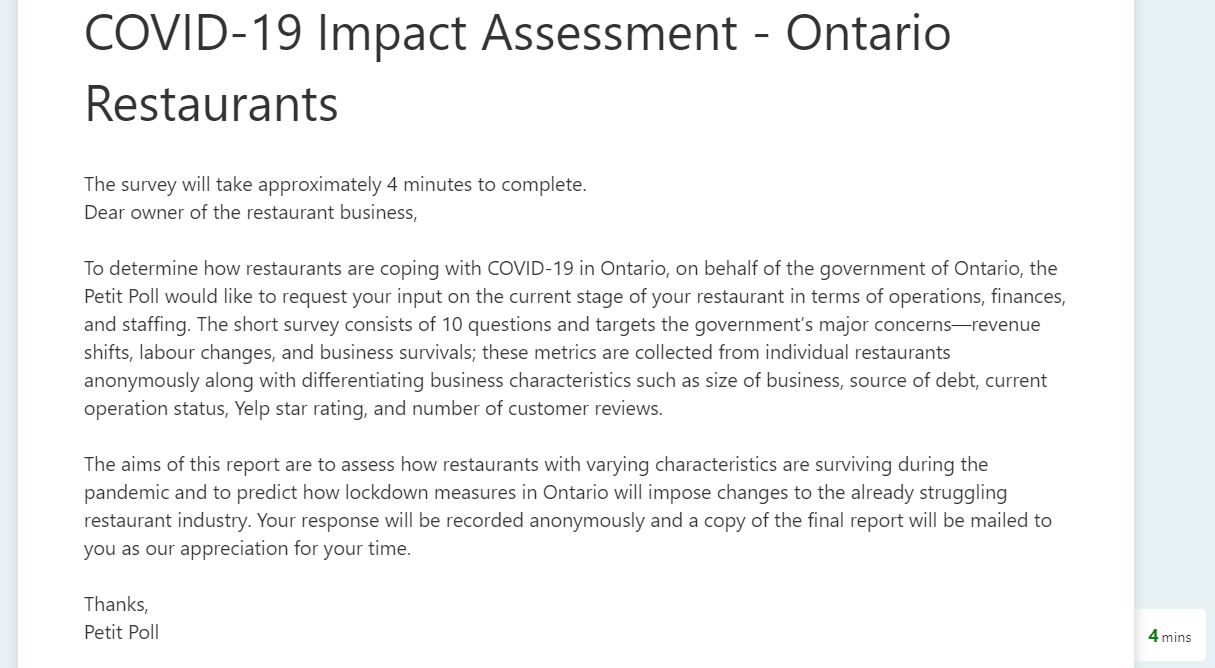
\includegraphics{"../../inputs/survey_opening.png"}
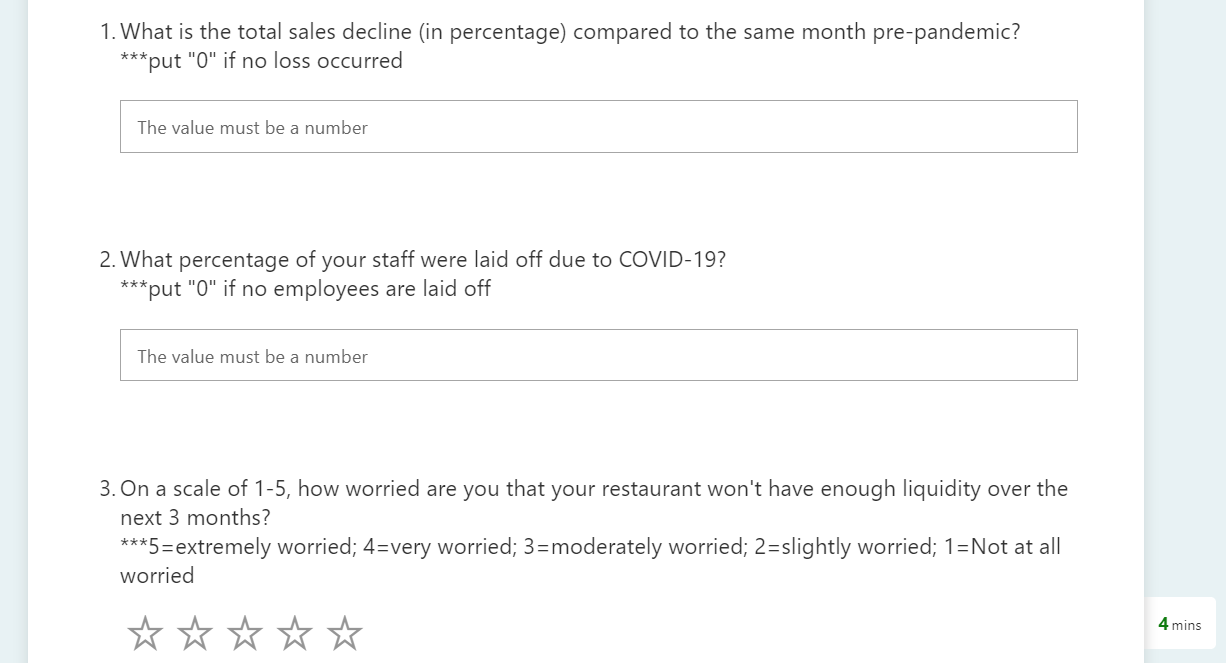
\includegraphics{"../../inputs/survey_topline.png"}
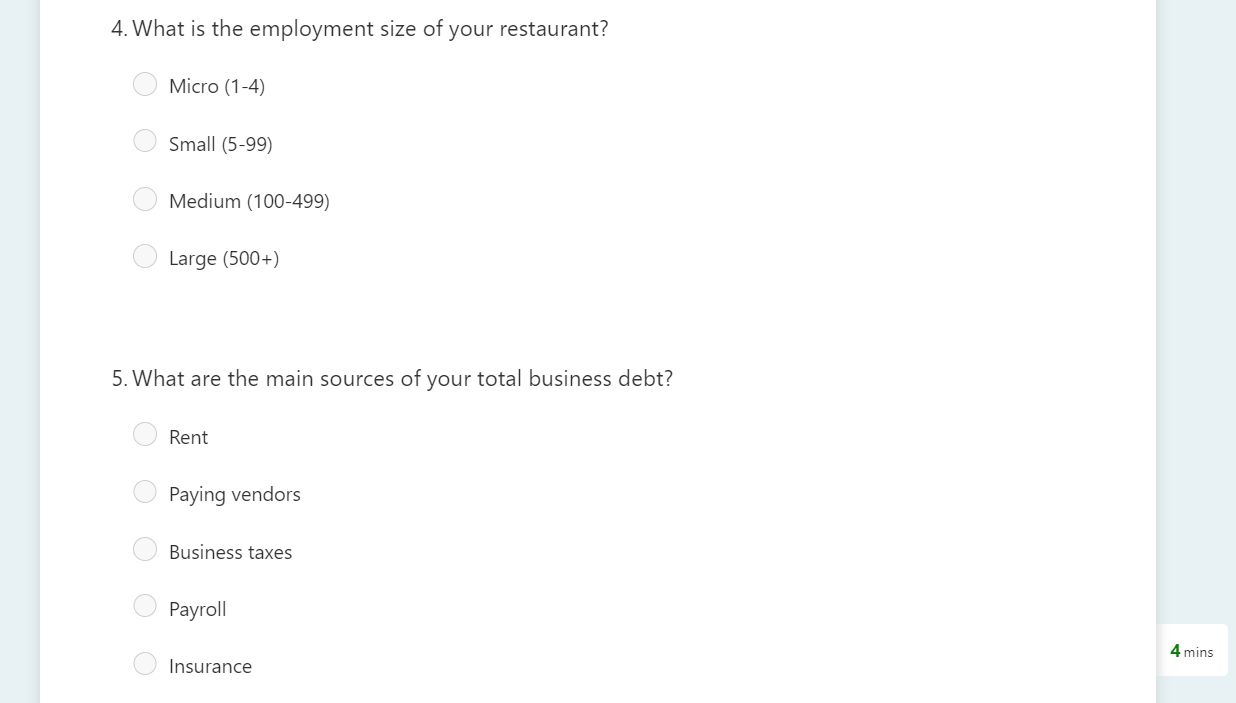
\includegraphics{"../../inputs/survey_q4_q5.png"}
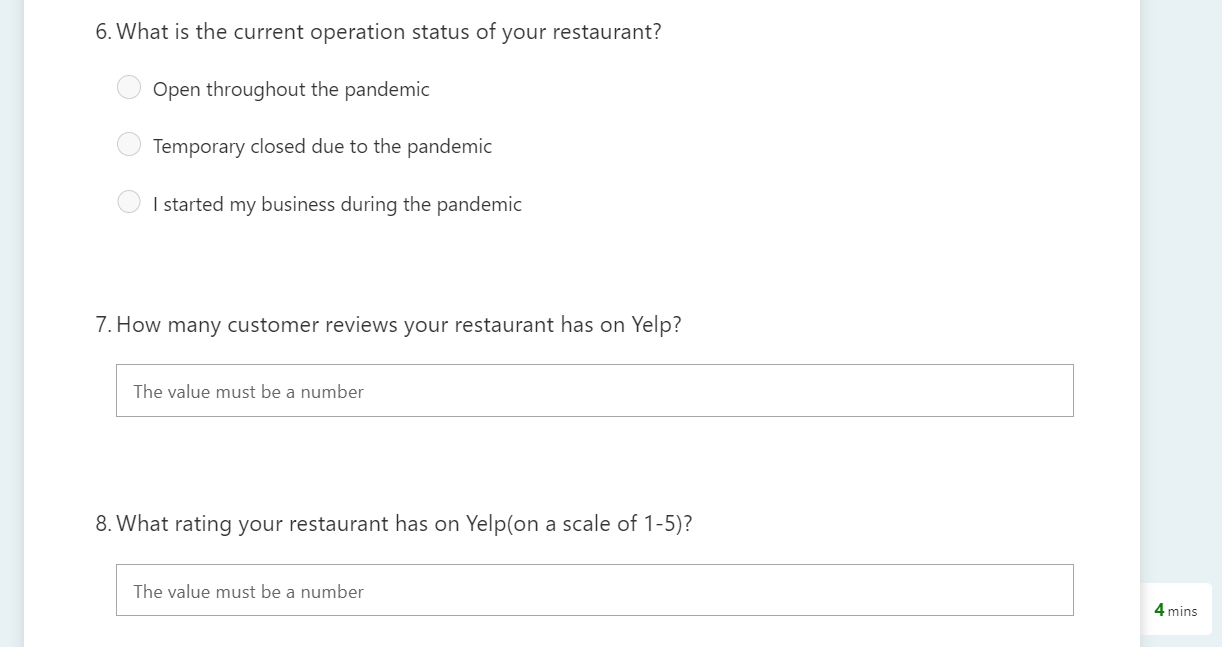
\includegraphics{"../../inputs/survey_q6_q7_q8.png"}
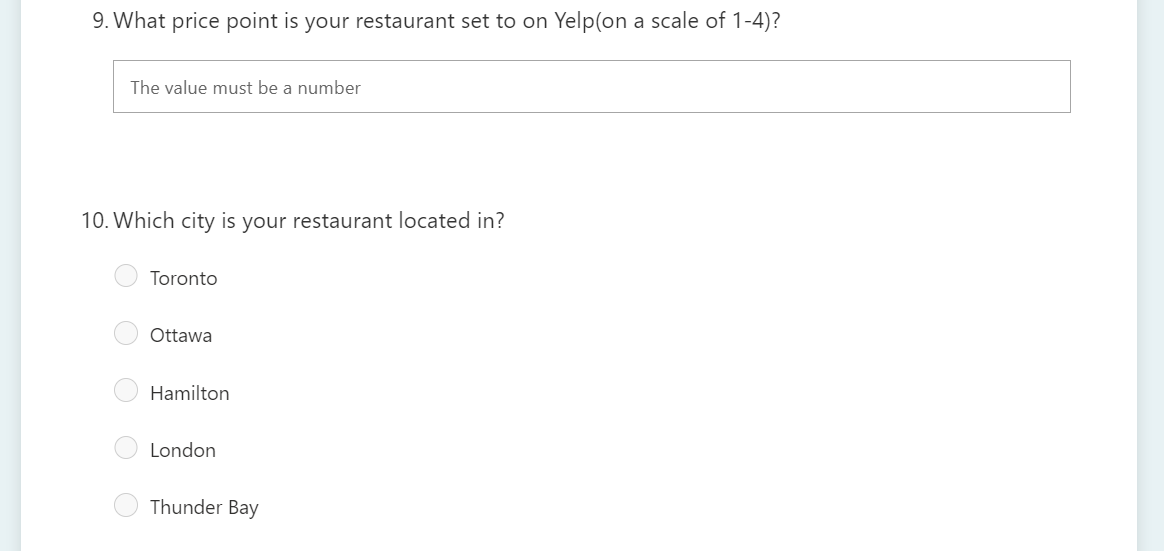
\includegraphics{"../../inputs/survey_q9_q10.png"}

\newpage

\hypertarget{references}{%
\section*{References}\label{references}}
\addcontentsline{toc}{section}{References}

\hypertarget{refs}{}
\begin{CSLReferences}{1}{0}
\leavevmode\hypertarget{ref-Samplesize}{}%
BYJU's. 2021. \emph{Sample Size Formula}. \url{https://byjus.com/sample-size-formula/}.

\leavevmode\hypertarget{ref-govCan}{}%
Canada, Government of. 2021. \emph{Businesses - Canadian Industry Statistics}. \url{https://www.ic.gc.ca/app/scr/app/cis/businesses-entreprises/72}.

\leavevmode\hypertarget{ref-restCan}{}%
Canada, Restaurant. 2020. \emph{Operations Report 2020}. \url{https://members.restaurantscanada.org/2020/06/26/operations-report/}.

\leavevmode\hypertarget{ref-RData}{}%
Canada, Statistics. 2020. \emph{Monthly Survey of Food Services and Drinking Plances}. \url{https://www150.statcan.gc.ca/t1/tbl1/en/tv.action?pid=2110001901}.

\leavevmode\hypertarget{ref-yelpCan}{}%
First Wave, Toronto After the. 2021. \emph{Disruptions to Restaurants}. \url{https://torontoafterthefirstwave.com/dashboards/restaurants/}.

\leavevmode\hypertarget{ref-citeLit6}{}%
Information, and Privacy Commissioner of Ontario. 2015. {``Best Practices for Protecting Individual Privacy in Conducting Survey Research.''}

\leavevmode\hypertarget{ref-citeLit7}{}%
Paul J. Gertler, Patrick Premand, Sebastian Martinez. 2016. {``Impact Evaluation in Practice.''}

\leavevmode\hypertarget{ref-citeLit1}{}%
Yang Yang, \& Hongbo Liu, Xiang Chen. 2020. {``COVID-19 and Restaurant Demand: Early Effects of the Pandemic and Stay-Athome Orders.''} \emph{International Journal of Contemporary Hospitality Management}.

\end{CSLReferences}

\end{document}
